\section{Desarrollo}

\subsection{PARTE I: Instalación Hyper-V}

\textbf {4.1.1. Verificar Edición de Windows 10:} El Hyper V es una característica de Windows 10 en las versiones PRO y Educational, para esto primero verificaremos si nuestro sistema pertenece a alguna de esas ediciones.
\begin{center}
  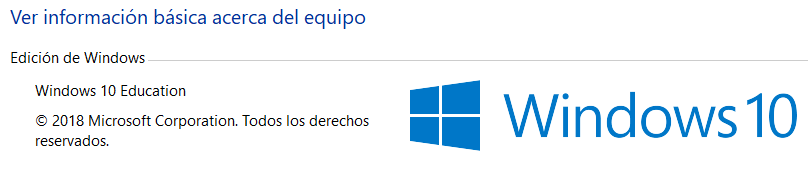
\includegraphics[width=15cm]{Imagenes/Windows_Education.png}
\end{center}

\textbf {4.1.2. Buscar la opción de Características de Windows:} Nos dirigimos al Menu del Windows 10 y buscamos la opción de "Activar o desactivar las caracterísitcas de Windows".\\
\begin{center}
  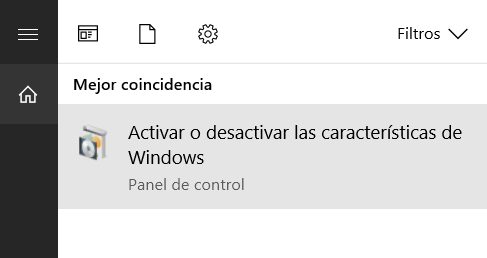
\includegraphics[width=15cm]{Imagenes/Activar_Caracteristicas.png}
\end{center}
\break

\textbf {4.1.3. Activar Característica Hyper-V:} Buscamos la opción llamada "Hyper V" y lo activamos.\\
\begin{center}
  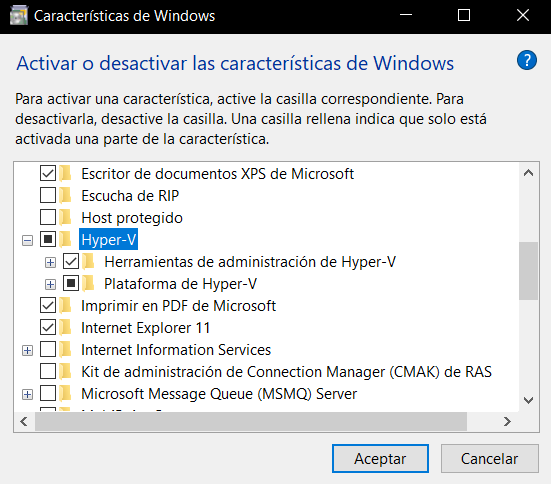
\includegraphics[width=11cm]{Imagenes/Activar_Hyper_V.png}
\end{center}

\textbf {4.1.4. Reiniciar el Sistema Operativo:} Con la finalidad de que se apliquen los cambios, es necesario reiniciar el equipo.
\begin{center}
  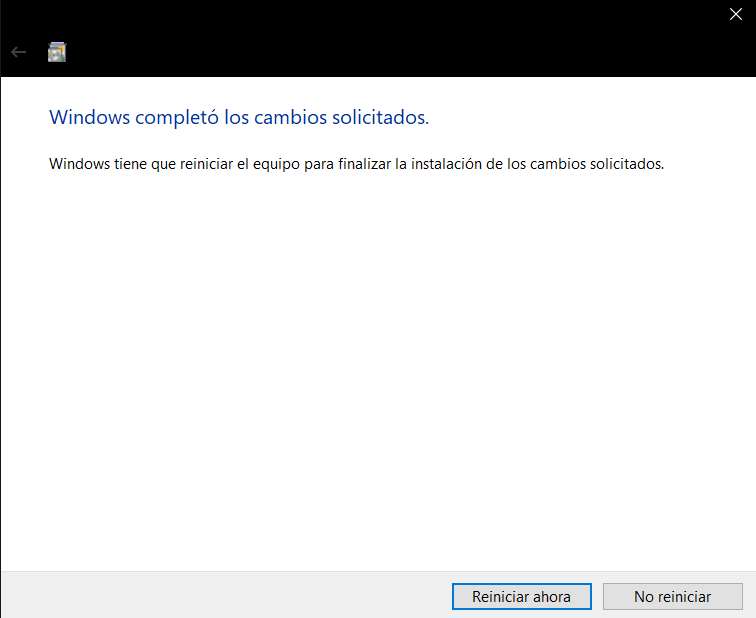
\includegraphics[width=11cm]{Imagenes/Reiniciar.png}
\end{center}
\break

\textbf {4.1.5. Hyper V correctamente habilitado:} Una vez reiniciada la computadora, ya podremos abrir nuestro Hyper-V que estará listo para ser configurada.\\
\begin{center}
  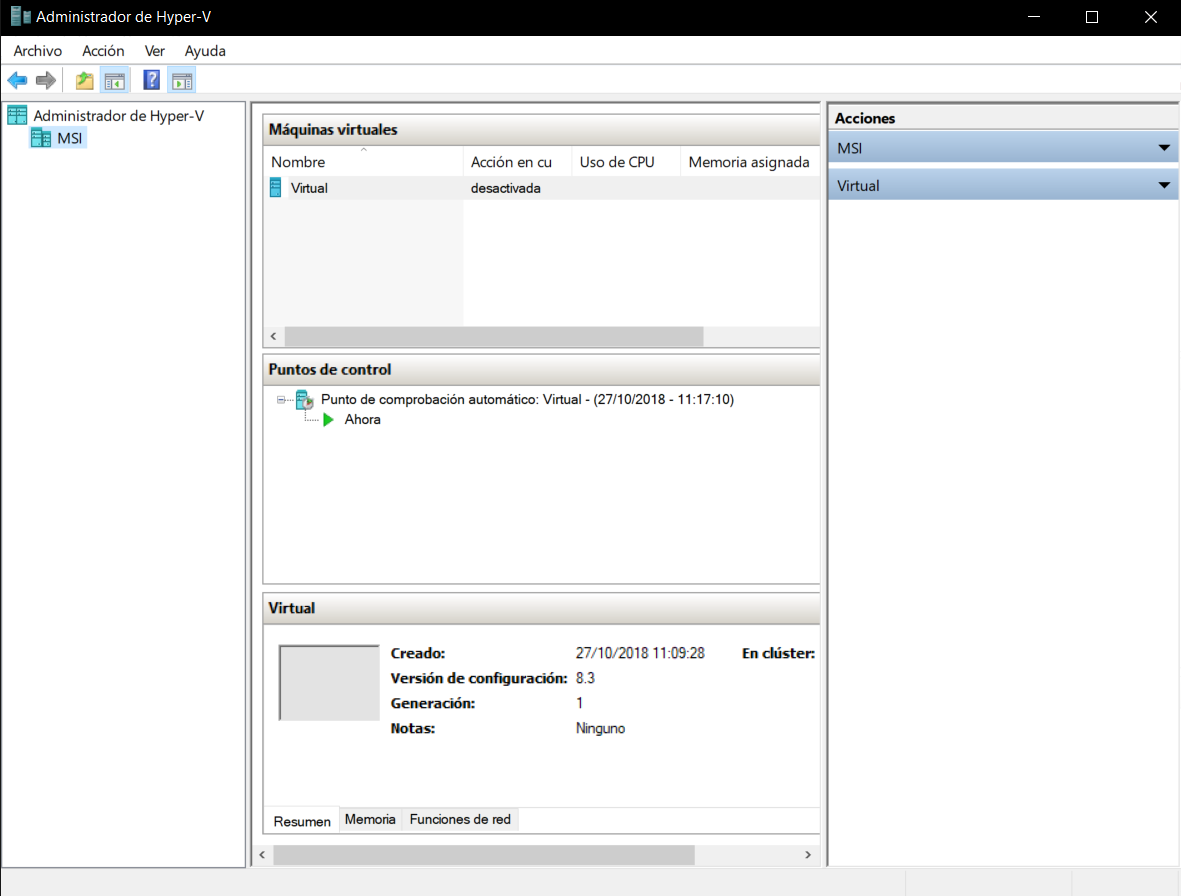
\includegraphics[width=14cm]{Imagenes/Hyper_V.png}
\end{center}
\break

\subsection{PARTE II: Instalación Windows Server 2016}

\textbf {4.2.1. Crear Nueva maquina Virtual:} En este paso crearemos una nueva maquina virtual donde instalaremos nuestro Windows Server 2016, para eso le daremos clic derecho a nuestro servidor de HYPER V.
\begin{center}
  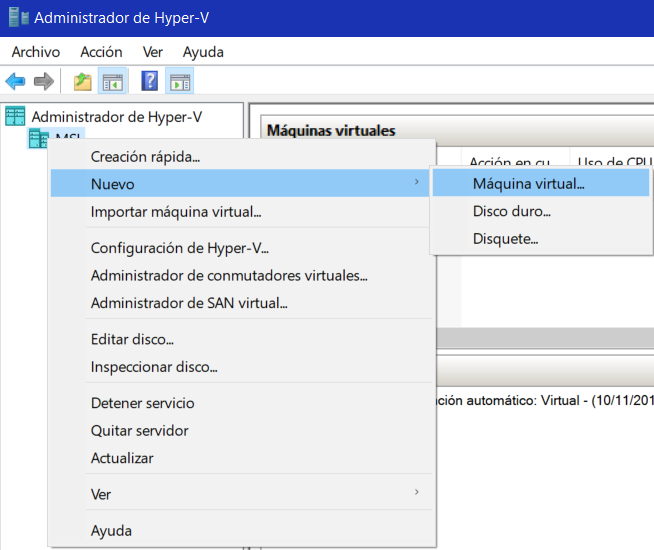
\includegraphics[width=11cm]{Imagenes/Nueva_Maquina.png}
\end{center}

\textbf {4.2.2. Especificar Nombre:} Ahora especificaremos el nombre de nuestra maquina virtual, en este caso le colocaremos Windows Server 2016.
\begin{center}
  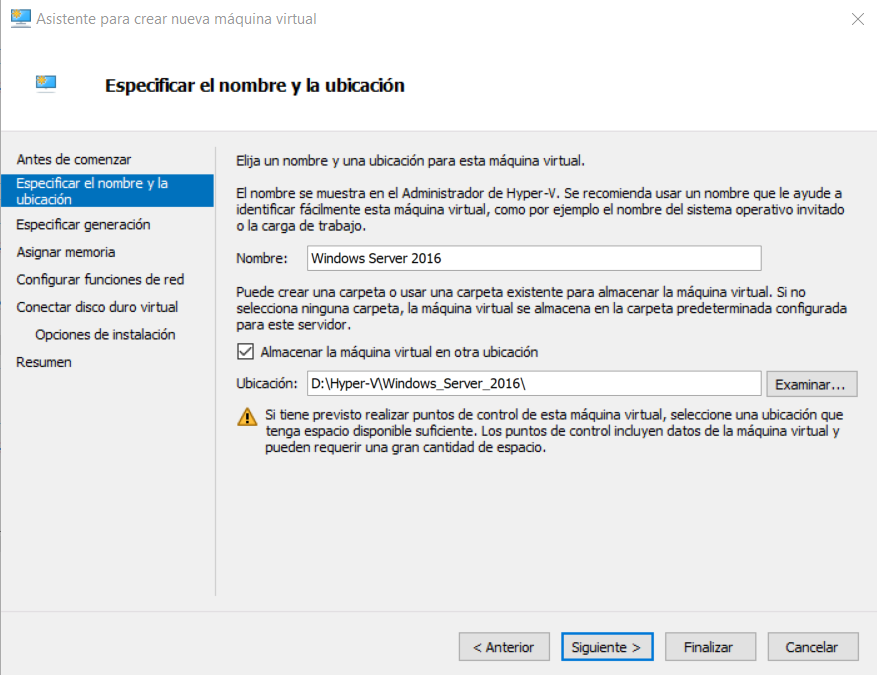
\includegraphics[width=11cm]{Imagenes/Especificar_Nombre_Ruta.png}
\end{center}
\break

\textbf {4.2.3. Elegir Generación:} Elegiremos la Generación que se marca por defecto, en este caso es la Generación 1.
\begin{center}
  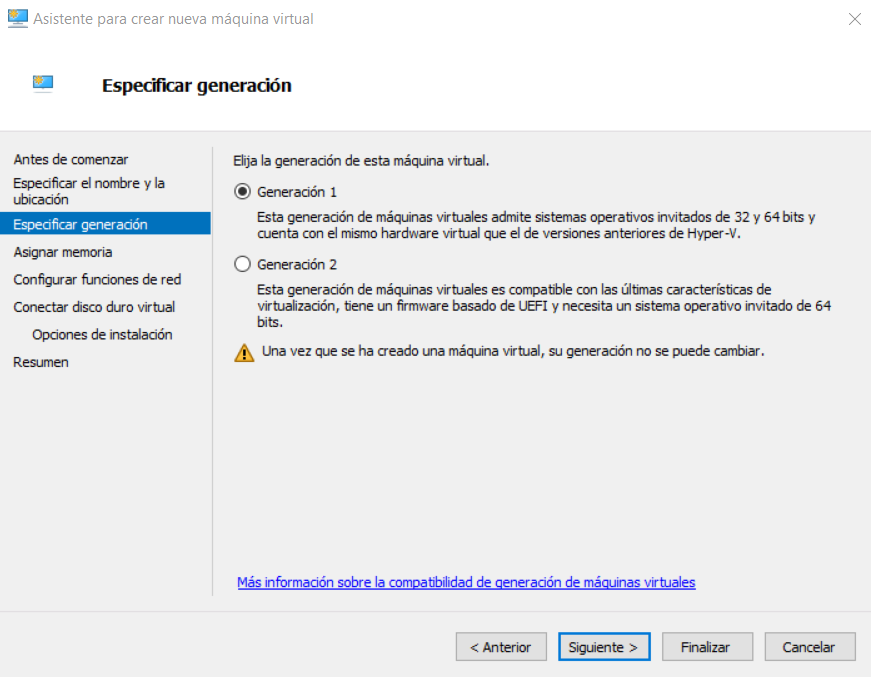
\includegraphics[width=11cm]{Imagenes/Especificar_Generacion.png}
\end{center}

\textbf {4.2.4. Asignar Memoria:} Elegiremos la cantidad de memoria con la que queremos que trabaje nuestra maquina virtual, en este caso le pusimos 2048mb y le damos clic en Siguiente.
\begin{center}
  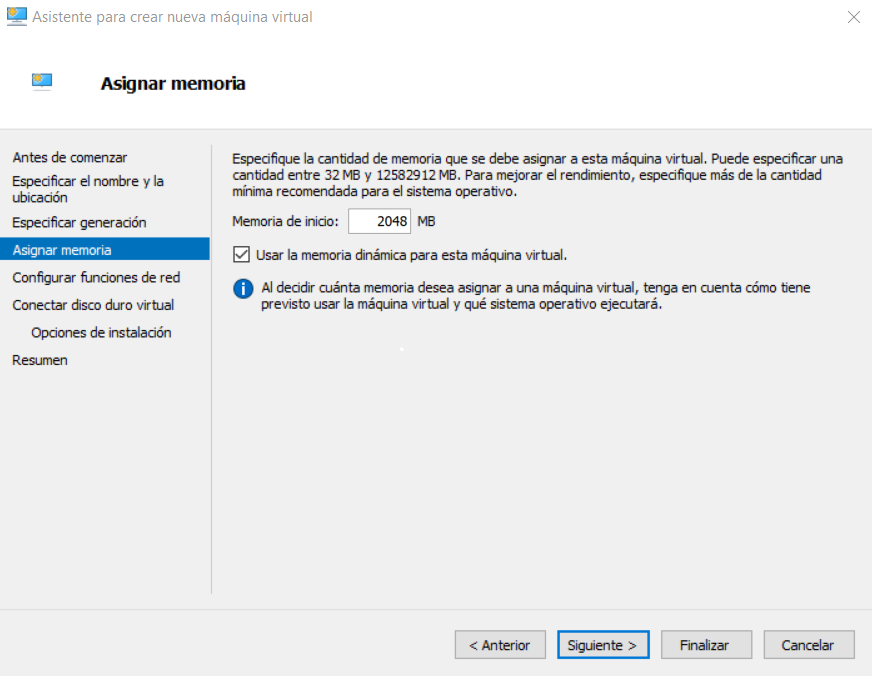
\includegraphics[width=11cm]{Imagenes/Asignar_Memoria.png}
\end{center}
\break

\textbf {4.2.5. Conectar Disco:} Estableceremos la ruta de nuestra maquina virtual y le asignaremos el tamaño de 80GB.
\begin{center}
  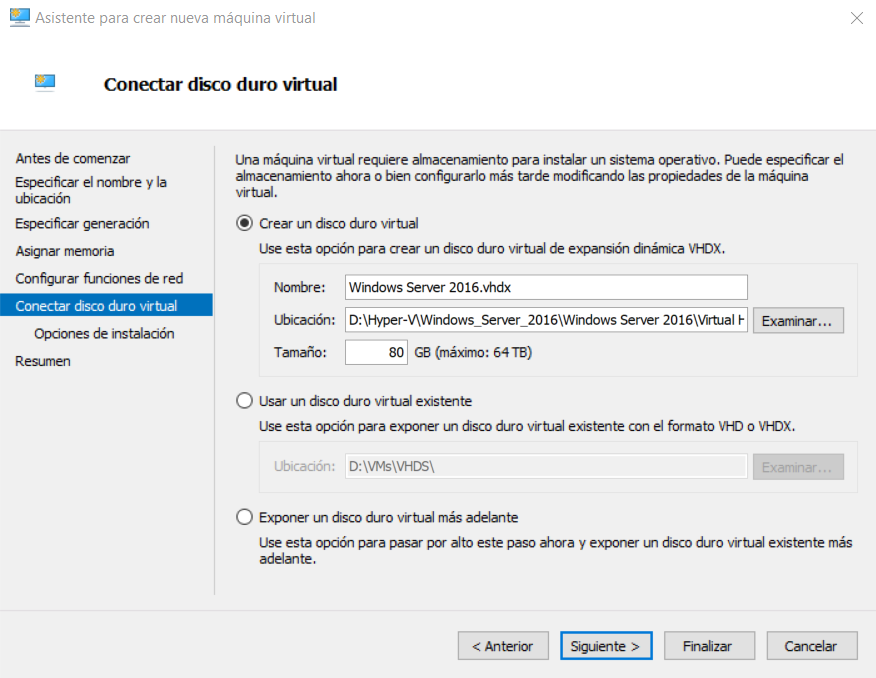
\includegraphics[width=11cm]{Imagenes/Conectar_Disco.png}
\end{center}

\textbf {4.2.6. Resumen:} Al terminar con la configuración, el asistente nos mostrará un Resumen de nuestra máquina virtual, si todo esta conforme le daremos clic en FINALIZAR.
\begin{center}
  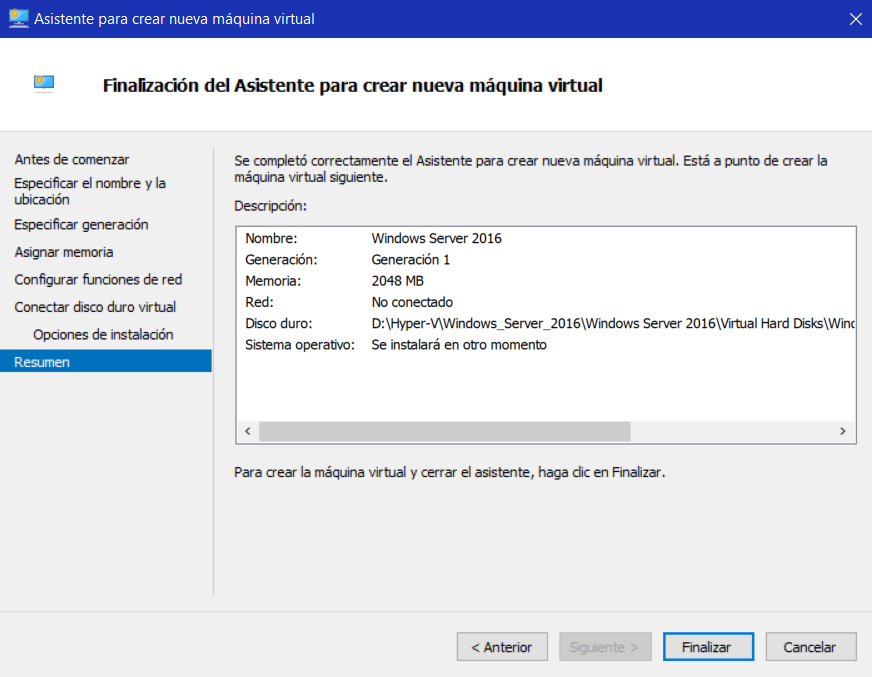
\includegraphics[width=11cm]{Imagenes/Resumen.png}
\end{center}
\break

\textbf {4.2.7. Conectar con la Máquina Virtual:}Para este paso le daremos clic derecho sobre nuestra máquina virtual y le damos clic en Conectar.
\begin{center}
  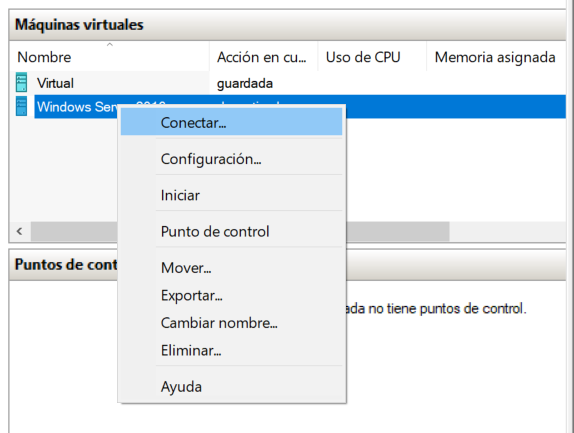
\includegraphics[width=11cm]{Imagenes/Conectar_WindowsServer.png}
\end{center}

\textbf {4.2.8. Iniciar Virtualización:} Una vez que hayamos conectado nuestra máquina virtual, se nos abrirá el virtualizador, nosotros le daremos clic en INICIAR, para que comience a virtualizar.
\begin{center}
  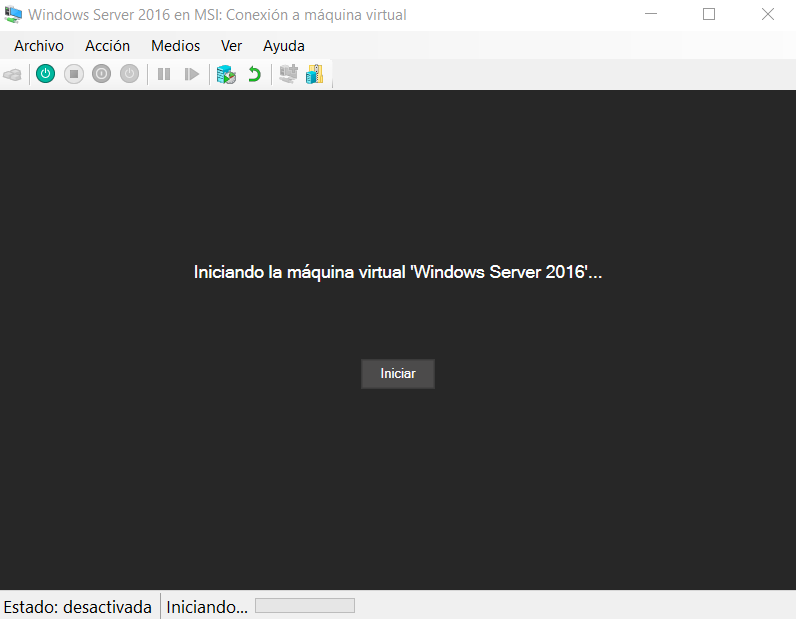
\includegraphics[width=11cm]{Imagenes/Iniciar_Virtualizacion.png}
\end{center}
\break

\textbf {4.2.9. Elegir el ISO de instalación:}Para este paso le daremos clic en Medios - Unidad de DVD y seleccionaremos la nuestro ISO.
\begin{center}
  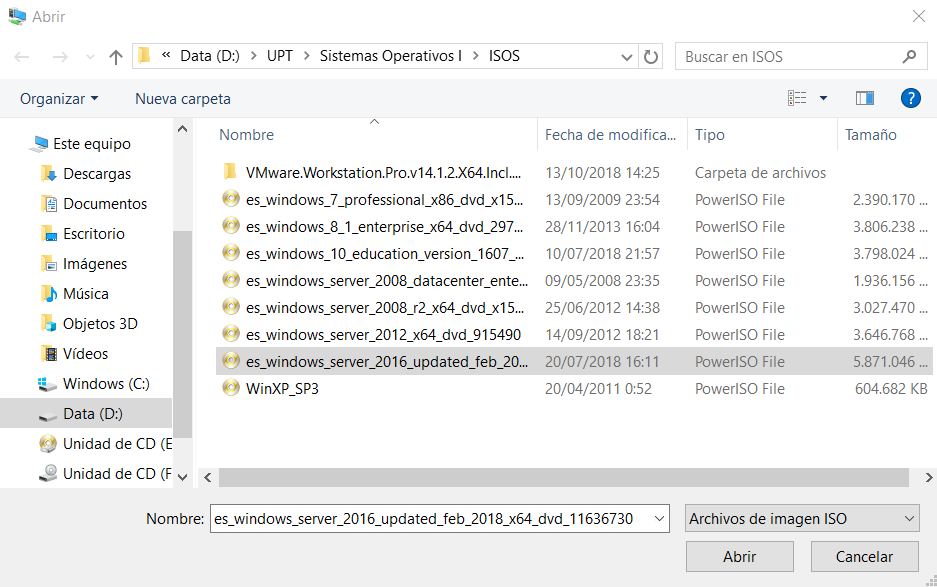
\includegraphics[width=11cm]{Imagenes/Elegir_ISO.png}
\end{center}

\textbf {4.2.10. Iniciar Instalación:} Luego de elegir nuestro ISO, volveremos a Iniciar nuestra Virtualización seguidamente nos aparecerá el cuadro de Instalación de Windows Server.
\begin{center}
  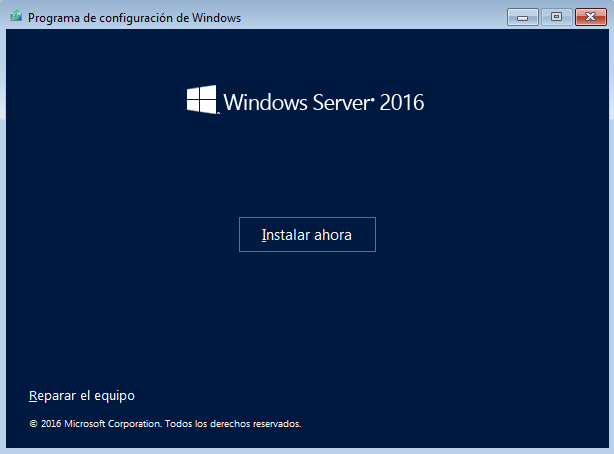
\includegraphics[width=11cm]{Imagenes/Instalar_Ahora.png}
\end{center}
\break

\textbf {4.2.11. Configuración de la Instalación:} Luego de hacer clic en Instalar Ahora, nos aparecera un cuadro donde podremos elegir el tipo de Idioma que deseamos usar en nuestro Windows Server, nosotros elegiremos Español Perú y le daremos clic en Siguiente.
\begin{center}
  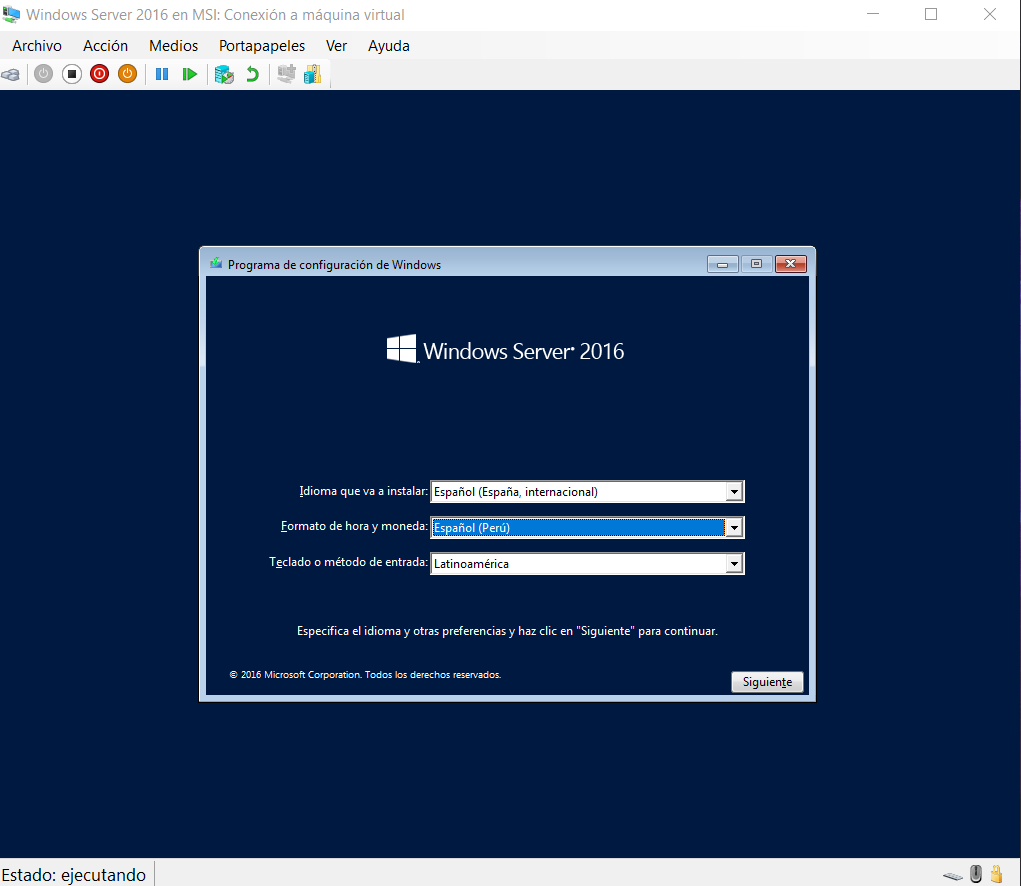
\includegraphics[width=11cm]{Imagenes/Iniciar_Instalacion.png}
\end{center}

\textbf {4.2.12. Ingresar Serial:} Si hemos comprado el software, debemos ingresar el Serial que llega junto al Instalador, en caso de no tener el Serial le damos clic en la opción: No tengo Clave del Producto y Siguiente.
\begin{center}
  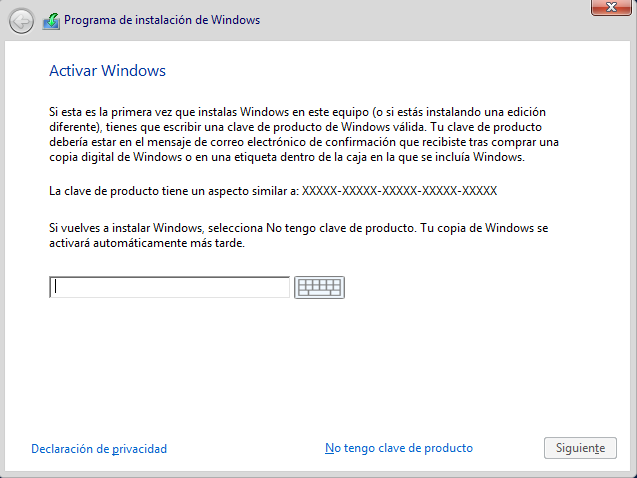
\includegraphics[width=11cm]{Imagenes/Ingresar_Serial.png}
\end{center}
\break

\textbf {4.2.13. Elegir Versión:} Elegiremos la opción de Windows Server 2016 DataCenter (Experiencia de Escritorio) y le damos clic en Siguiente
\begin{center}
  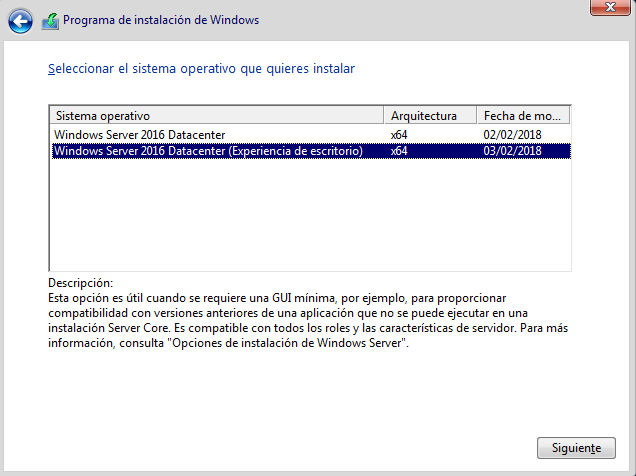
\includegraphics[width=11cm]{Imagenes/Elegir_Version.png}
\end{center}

\textbf {4.2.14. Aceptar Licencia:} Leeremos los términos y licencia y activaremos el check de ACEPTO, y luego clic en Siguiente.
\begin{center}
  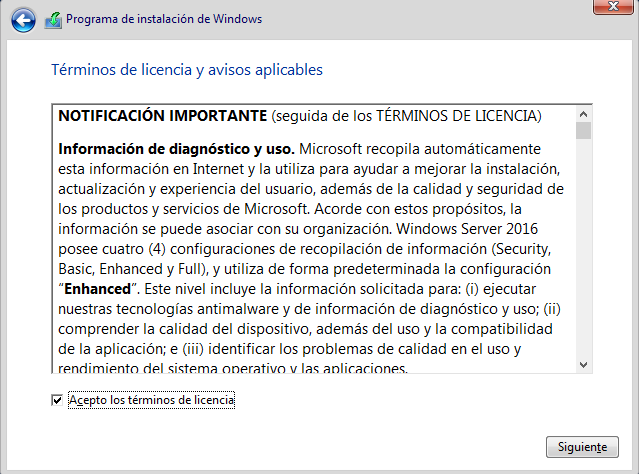
\includegraphics[width=11cm]{Imagenes/Aceptar_Licencia.png}
\end{center}
\break

\textbf {4.2.15. Tipo de Instalación:} Nosotros le daremos clic en Instalación Personalizada.
\begin{center}
  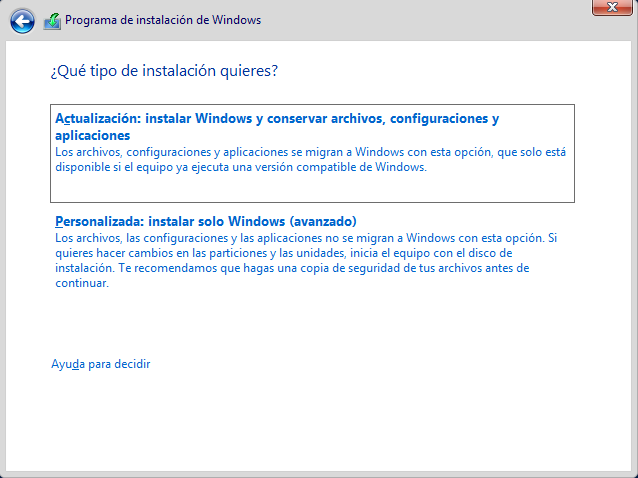
\includegraphics[width=11cm]{Imagenes/Elegir_Tipo_Instalacion.png}
\end{center}

\textbf {4.2.16. Disco de Instalación:} Elegiremos el único disco disponible (Unidad 0) y le daremos clic en Siguiente.
\begin{center}
  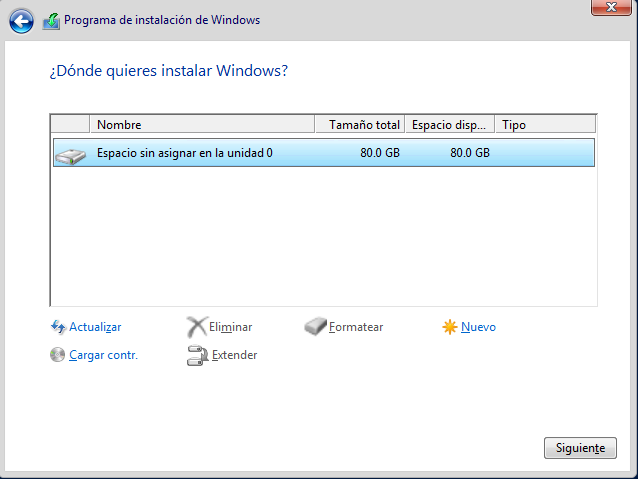
\includegraphics[width=11cm]{Imagenes/Elegir_Disco_Instalacion.png}
\end{center}
\break

\textbf {4.2.17. Proceso de Instalacion:} Luego comenzará la Instalación de nuestro Windows Server, en este paso solo queda esperar a que la Instalación termine.
\begin{center}
  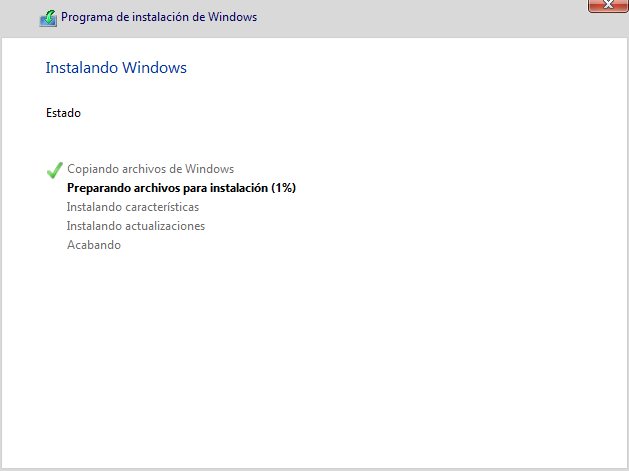
\includegraphics[width=11cm]{Imagenes/Proceso_Instalacion.png}
\end{center}

\textbf {4.2.18. Crear Clave:} Luego de que el Proceso de Instalación haya terminado, ahora debemos crear una clave para el Administrador del Servidor, en este caso nosotros le asignaremos la clave de: Sistemas.2018
\begin{center}
  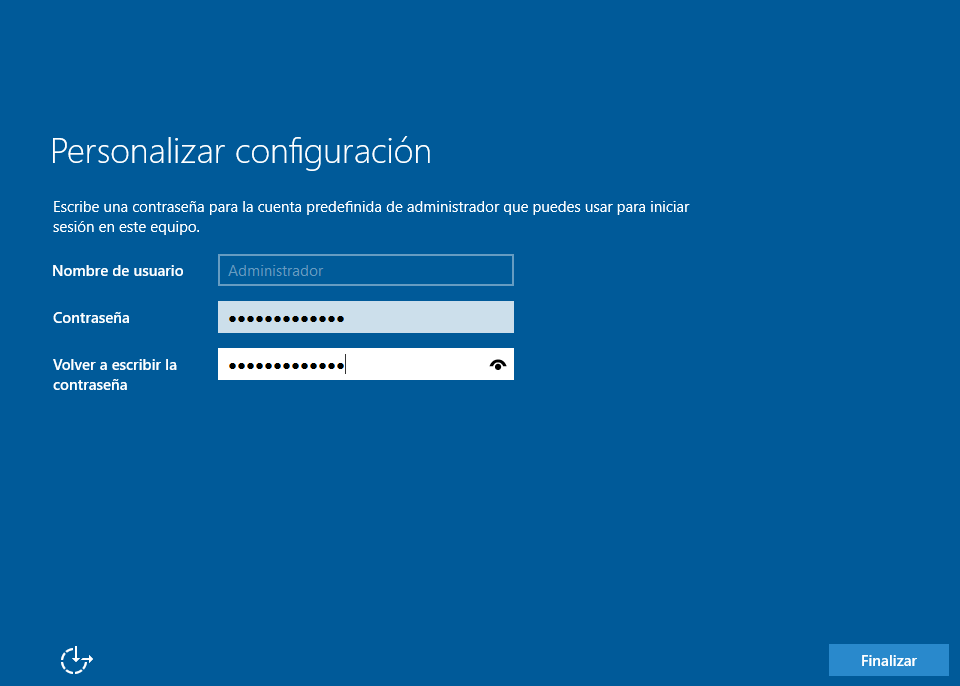
\includegraphics[width=11cm]{Imagenes/Crear_Clave.png}
\end{center}
\break

\textbf {4.2.19. Identificarse en el Windows Server:} En este paso debemos identificarnos para poder iniciar nuestro Windows Server, para esto ingresaremos con la contraseña antes creada: Sistemas.2018
\begin{center}
  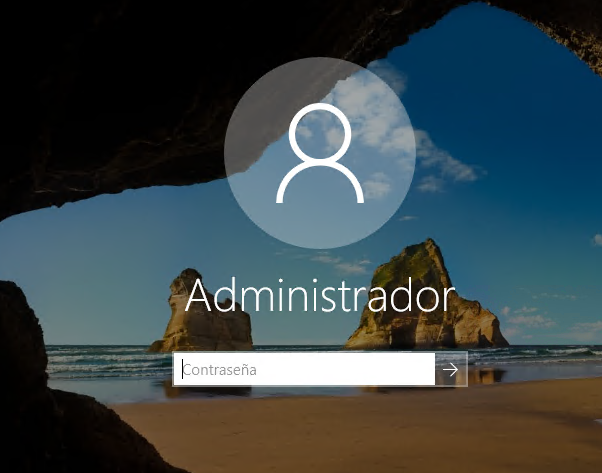
\includegraphics[width=11cm]{Imagenes/Identificarse.png}
\end{center}

\textbf {4.2.20. Windows Server 2016:} Luego de tanta espera, al fin podremos acceder a nuestro Windows Server la cuál se encuentra lista para poder instalarle el Oracle DataBase.
\begin{center}
  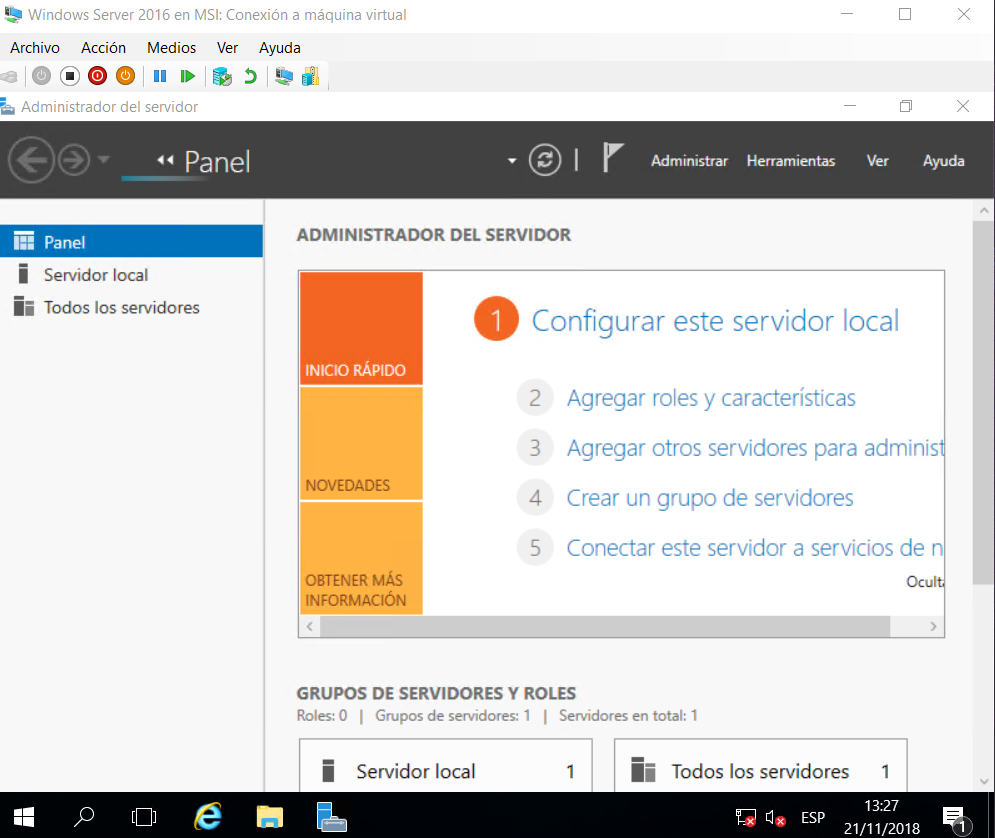
\includegraphics[width=11cm]{Imagenes/Escritorio_Windows_Server.png}
\end{center}
\break